\documentclass[slides,aspectratio=169]{beamer}
% compile with lualatex --shell-escape presentation.tex

% Metropolis theme with Imperial colors
\useoutertheme[progressbar=foot]{metropolis}
\useinnertheme{metropolis}
\usefonttheme{metropolis}
\usecolortheme{metropolis}
\usecolortheme{imperial}
% \usefonttheme[onlymath]{serif}
\usepackage{listings}
\usepackage{shellesc}

% Math stuff
\usepackage{bm}
\usepackage{bbm}         % Blackboard fonts
\usepackage{amsmath}
\usepackage{mathtools}
\usepackage{commath}

% Citations and references
\usepackage{natbib}
\usepackage{hyperref}
%\usepackage[natbib, maxcitenames=3, mincitenames=1, style=apa]{biblatex}
% Language and input
\usepackage[english]{babel}
\usepackage[utf8x]{inputenc}

% tikz and pgfplots
\usepackage{xcolor}
\usepackage{pgfplots,tikz}
\usetikzlibrary{shapes.geometric,arrows,positioning}
\usetikzlibrary{external}
\tikzexternalize[optimize=false,prefix=tikz/]

\usepackage{graphicx}
\usepackage{datetime}
%\usepackage[T1]{fontenc}
\usepackage{listings}
% \usepackage{color}
\usepackage{multirow,multicol,booktabs}
\usepackage{makecell}
\usepackage{adjustbox}
\usepackage{tabto}

% Algorithms
\usepackage{algorithmic}
\usepackage{algorithm}

\newcommand{\isoSpacing}{\ \ \ \ \ \ \ \ \ \ }
\setlength{\abovedisplayskip}{-5pt}
\setlength{\belowdisplayskip}{-5pt}
\setlength{\abovedisplayshortskip}{-5pt}
\setlength{\belowdisplayshortskip}{-5pt}

\setbeamertemplate{footline}
  {
    \leavevmode%
    \hbox{%
    \begin{beamercolorbox}[wd=.35\paperwidth,ht=2.25ex,dp=1ex,center]{author}%
      \usebeamerfont{author in head/foot}\insertshortauthor
    \end{beamercolorbox}%
    \begin{beamercolorbox}[wd=.3\paperwidth,ht=2.25ex,dp=1ex,center]{title}%
      \usebeamerfont{title in head/foot}\insertshorttitle
    \end{beamercolorbox}%
    \begin{beamercolorbox}[wd=.35\paperwidth,ht=2.25ex,dp=1ex,right]{date}%
        \usebeamerfont{date in
        head/foot}\insertshortinstitute\hspace*{3ex}\phantom{10}\makebox[0pt][r]{\insertframenumber{}} /
    \insertmainframenumber\hspace*{1ex}
    \end{beamercolorbox}}%
    \vskip0pt%
  }



\definecolor{codegreen}{rgb}{0,0.6,0}
\definecolor{codegray}{rgb}{0.5,0.5,0.5}
\definecolor{codepurple}{rgb}{0.58,0,0.82}
\definecolor{backcolour}{rgb}{0.95,0.95,0.92}

\lstdefinestyle{python}{
    backgroundcolor=\color{backcolour},
    commentstyle=\color{codegreen},
    keywordstyle=\color{magenta},
    numberstyle=\tiny\color{codegray},
    stringstyle=\color{codepurple},
    basicstyle=\ttfamily\footnotesize,
    breakatwhitespace=false,
    breaklines=true,
    captionpos=b,
    keepspaces=true,
    numbers=left,
    numbersep=5pt,
    showspaces=false,
    showstringspaces=false,
    showtabs=false,
    tabsize=2
}

\lstset{style=python}
\renewcommand{\vec}{\boldsymbol}
\newcommand{\x}{\vec{x}}
\newcommand{\yi}{\vec{y}_i}
\newcommand{\X}{\mathcal{X}}
%\spnewtheorem{algorithm}{Algorithm}{\bf}{\rm}

\renewcommand{\vec}{\boldsymbol}
\newcommand{\y}{\vec{y}}
\newcommand{\R}{\mathbb{R}}
\newcommand{\U}{\mathcal{U}}
\newcommand{\Ueps}{\mathcal{U}^{\alpha}}
\newcommand{\E}{\mathcal{E}^{\alpha}}
\newcommand{\muvec}{\vec{\mu}}
\newcommand{\z}{\vec{z}}
\newcommand{\avec}{\vec{a}}
\newcommand{\T}{^\intercal}
\newcommand{\gunc}{\tilde{g}}
\newcommand{\aunc}{\tilde{a}}
\newcommand{\punc}{\tilde{p}}
\newcommand{\Ue}{\U^{\mathcal{E}}}
\newcommand{\covm}{\vec{\Sigma}}
\newcommand{\zstar}{\vec{z}^*}
\newcommand{\ystar}{\vec{y}^*}
\newcommand{\zhat}{\vec{\hat{z}}}
\newcommand{\cvec}{\vec{c}}
\newcommand{\dz}{\vec{\Delta z}}
\newcommand{\dzhat}{\vec{\Delta \hat{z}}}
\newcommand{\N}{\mathbb{N}}
\newcommand{\cU}{c(\U)}
\newcommand{\Q}{\mathcal{Q}}
\newcommand{\A}{\mathcal{E}^\alpha}
\newcommand{\B}{\mathcal{B}^\alpha}
\newcommand{\xton}{\y_1, \ldots, \y_n}
\newcommand{\xtol}{\y_1, \ldots, \y_l}
\newcommand{\xstarton}{\y^*_i : i \in [n]}
\newcommand{\xstartol}{\y^*_1, \ldots, \x^*_l}
% \newcommand{\Aton}{\A(\xton)}
\newcommand{\Aton}{\A(\y)}
\newcommand{\Uton}{\U(\y)}
\newcommand{\Atol}{\A(\xtol)}
\newcommand{\Bton}{\B(\xton, \lambda)}
\newcommand{\lammax}{\lambda_{\text{max}}}
\newcommand{\lammin}{\lambda_{\text{min}}}
\newcommand{\signoise}{\sigma_{\text{noise}}}
\newcommand{\fix}{}
% \newcommand{\fix}{\color{orange}}
% \newcommand{\citet}[1]{\citeauthor{#1} \shortcite{#1}}
\newcommand{\Hinv}{\h^{-1}}
\DeclarePairedDelimiter\ceil{\lceil}{\rceil}
\DeclarePairedDelimiter\floor{\lfloor}{\rfloor}
\newcommand{\Fn}{F_n^{1-\alpha}}
\DeclareMathOperator*{\argmin}{arg\min}
\DeclareMathOperator*{\argmax}{arg\max}
\newcommand{\h}{\boldsymbol{h}}
\newcommand{\GP}{\mathcal{GP}}

% DRILLING
\newcommand{\xstart}{{x_{0}}}
\newcommand{\xfin}{{x_n}}
\newcommand{\Dx}{{\Delta x}}
\newcommand{\Dp}{{\Delta p}}
\newcommand{\Dt}{{\Delta t}}
\newcommand{\Ndottop}{\dot{N}}
\newcommand{\Ndottopi}{\dot{N}_{i}}
\newcommand{\Ndotbit}{\dot{N}_\text{bit}}
\newcommand{\NdotPDM}{\dot{N}_\text{PDM}}
\newcommand{\cdrill}{c_\text{drill}}
\newcommand{\cmaint}{c_\text{maint}}

\NewDocumentCommand{\grad}{e{_^}}{%
  \mathop{}\!% \mathop for good spacing before \nabla
  \nabla
  \IfValueT{#1}{_{\!#1}}% tuck in the subscript
  \IfValueT{#2}{^{#2}}% possible superscript
}

\newcommand{\xivec}{\vec{\xi}}
\newcommand{\xixi}{(\underbar{\xivec}, \bar{\xivec})}

%\setsansfont[BoldFont={Fira Sans}, ItalicFont={Fira Sans Light Italic}]{Fira Sans Light}
\title[ROmodel]{\vspace{5pt} ROmodel: Modeling robust optimization problems in
Pyomo\vspace{-10pt}}

% Ines and Ruth as co-authors
    \author[J. Wiebe et al.]{Johannes Wiebe\inst{1}, Ruth Misener\inst{1}}
\institute[Imperial College London]{
    \vspace{10pt}
    \inst{1} Department of Computing, Imperial College London, London, UK\\[2em]
    \tiny
    Funding: EP/L016796/1, EP/R511961/1 no. 17000145, and EP/P016871/1
}

\newdate{date}{07}{06}{2021}
\date{\displaydate{date}}

\begin{document}

\tikzexternaldisable
\begin{frame}[noframenumbering,plain]
  \begin{tikzpicture}[overlay, remember picture]
  \node[anchor=north west, %anchor is upper left corner of the graphic
      xshift=7pt, %shifting around
      yshift=-6pt]
     at (current page.north west) %left upper corner of the page
     {
\includegraphics[width=0.29\textwidth]{img/logo_imperial.eps}};
  \end{tikzpicture}
  \begin{tikzpicture}[overlay, remember picture]
  \node[anchor=north east, %anchor is upper left corner of the graphic
      xshift=-220pt, %shifting around
      yshift=-4pt]
     at (current page.north east) %left upper corner of the page
     {
\includegraphics[width=0.23\textwidth]{img/logo_cog.png}};
  \end{tikzpicture}
  \begin{tikzpicture}[overlay, remember picture]
  \node[anchor=north east, %anchor is upper left corner of the graphic
      xshift=-113pt, %shifting around
      yshift=-10pt]
     at (current page.north east) %left upper corner of the page
     {
\includegraphics[width=0.23\textwidth]{img/logo_hipeds.pdf}};
  \end{tikzpicture}
  \begin{tikzpicture}[overlay, remember picture]
  \node[anchor=north east, %anchor is upper left corner of the graphic
  xshift=-4pt, %shifting around
  yshift=-10pt]
  at (current page.north east) %left upper corner of the page
  {
\includegraphics[width=0.23\textwidth]{img/logo_slb.eps}};
  \end{tikzpicture}
    \maketitle
\end{frame}

% DO NOT put this before the title frame
\tikzexternalenable

\begin{frame}{Robust optimization}
Consider a generic robust optimization problem:
\begin{subequations}
    \begin{align}
        \min\limits_{\x\in \mathcal{X} , \y(\xivec)}\max\limits_{\xivec \in \U(\x)}\quad & f(\x, \y(\xivec), \xivec)  \\[4pt]
        \text{s.t} \quad & g(\x, \y(\xivec), \xivec) \leq 0 && \forall \xivec \in \U(\x)
    \end{align}\label{eq:ro}
\end{subequations}
where $\x \in \R^n$ are "here and now" variables, $\y(\xivec)$ are adjustable variables,
and the uncertain parameter vector $\xivec$ is bounded
by the uncertainty set $\U(\x)$.

\visible<2>{
    \begin{exampleblock}{Solution approaches}
        \begin{enumerate}
            \item Robust reformulation: based on duality
            \item Cutting planes: iterative approach
        \end{enumerate}
    \end{exampleblock}
}

\end{frame}

\begin{frame}{Existing tools}
    There are a number of existing tools for solving robust optimization
    problems:
    \begin{columns}
        \begin{column}{0.465\textwidth}
            \visible<2->{
            \begin{block}{Solvers}
                \vspace{1em}
                \begin{minipage}[c][0.30\textheight][t]{\linewidth} 
                Designed to \emph{solve} RO problems
                \begin{itemize}
                    \item ROME [1], RSOME [2]: Matlab
                    \item PyROS [3]: Python/Pyomo
                    \item ROC++ [4]: C++
                \end{itemize}
                \end{minipage}
            \end{block}
            }
        \end{column}
        \begin{column}{0.465\textwidth}
            \visible<3->{
            \begin{block}{Modeling languages}
                \vspace{1em}
                \begin{minipage}[c][0.30\textheight][t]{\linewidth} 
                Designed for \emph{modeling} RO problems
                    \begin{itemize}
                        \item JumPeR [5]: Julia/JumP
                        \item AIMMS
                    \end{itemize}
                \end{minipage}
            \end{block}
            }
        \end{column}
    \end{columns}
    \visible<4->{
    \begin{exampleblock}{ROmodel}
        Focuses on modeling. ROmodel is open source, tightly
        integrated with Pyomo, and allows modeling uncertainty sets with
        Pyomo constraints.
    \end{exampleblock}
    }
    \tiny
    [1] \cite{Goh2011},
    [2] \cite{Chen2020},
    [3] \cite{pyros},
    [4] \cite{Vayanos2020},
    [5] \cite{Dunning2016}
\end{frame}

\begin{frame}{New modeling objects}
    ROmodel introduces three new modeling components:
    \begin{itemize}
        \visible<2->{
        \item \lstinline{UncParam}: Similar to Pyomo's \lstinline{Var} or
            \lstinline{Param}; used to model uncertain parameters
        }\visible<3->{
        \item \lstinline{UncSet}: Based on Pyomo's \lstinline{Block} component;
            used to model uncertainty sets
        }\visible<4->{
        \item \lstinline{AdjustableVar}: Very similar to Pyomo's
            \lstinline{Var}; used for "wait and see" variables
        }
    \end{itemize}
    \visible<5->{
    These components can be used in Pyomo models like any Pyomo modeling
    component.  }
\end{frame}

\begin{frame}[fragile]{Modeling uncertain parameters}
    Uncertain parameters are the central component of robust optimization
    problems:
\begin{lstlisting}[language=Python]
    import pyomo.environ as pe
    import romodel as ro
    # Construct model
    m = pe.ConcreteModel()
    # Add uncertain parameters
    m.c = ro.UncParam(range(3), nominal=[0.1, 0.2, 0.3], uncset=m.U)
\end{lstlisting}
\visible<2->{
Arguments:
\begin{itemize}
    \item \lstinline{index}: (optional), \lstinline{UncParam} can be indexed or
        not
    \item \lstinline{nominal}: specifies nominal values for the uncertain
        parameters
    \item \lstinline{uncset}: specifies an uncertainty set for the uncertain
        parameters
\end{itemize}
}
\end{frame}

\begin{frame}[fragile]{Modeling uncertainty sets}
    Uncertainty sets can be specified in two ways:
    \begin{enumerate}
        \item Generic sets with Pyomo constraints
\begin{lstlisting}[language=Python]
    # Define uncertainty set & uncertain parameters
    m.U = ro.UncSet()
    m.c = UncParam(range(2), uncset=m.U, nominal=[0.5, 0.5])
    # Add constraints to uncertainty set
    m.U.cons1 = Constraint(expr=m.c[0] + m.c[1] <= 1)
    m.U.cons2 = Constraint(expr=m.c[0] - m.c[1] <= 1)
\end{lstlisting}
        \item Library sets
\begin{lstlisting}[language=Python]
    # Define polyhedral set
    m.U = ro.uncset.PolyhedralSet(rhs=[1, 1, 1, 1], mat=[[ 1,  1],
                                                         [ 1, -1],
                                                         [-1,  1],
                                                         [-1, -1]])
\end{lstlisting}
    \end{enumerate}
% \begin{lstlisting}[language=Python]
%     # Define ellipsoidal set
%     m.U = ro.uncset.EllipsoidalSet(cov=[[1, 0, 0],
%                               [0, 1, 0],
%                               [0, 0, 1]],
%                          mean=[0.5, 0.3, 0.1])
% \end{lstlisting}
\end{frame}

\begin{frame}[fragile]{Modeling uncertain constraints}
    Users can model uncertain constraints implicitly by using
    \lstinline{UncParam} objects in Pyomo constraints.

    Consider a deterministic Pyomo constraint:
\begin{lstlisting}[language=Python]
    # deterministic
    m.x = Var(range(3))
    c = [0.1, 0.2, 0.3]
    m.cons = Constraint(expr=sum(c[i]*m.x[i] for i in m.x) <= 0)
\end{lstlisting}
    If \lstinline{c} is uncertain, the robust formulation is:
\begin{lstlisting}[language=Python]
    # robust
    m.x = Var(range(3))
    m.c = UncParam(range(3), nominal=[0.1, 0.2, 0.3], uncset=m.U)
    m.cons = Constraint(expr=sum(m.c[i]*m.x[i] for i in m.x) <= 0)
\end{lstlisting}
\end{frame}

\begin{frame}[fragile]{Modeling adjustable variables}
    Adjustable variable: Decision variable who's value is determined after the
    uncertainty has been revealed.

    Defining adjustable variables in ROmodel with the \lstinline{AdjustableVar}
    class:
\begin{lstlisting}[language=Python]
    # Define uncertain parameters and adjustable variables
    m.w = UncParam(range(3), nominal=[1, 2, 3], uncset=m.U)
    m.y = AdjustableVar(range(3), uncparams=[m.w], bounds=(0, 1))
\end{lstlisting}
    Arguments \lstinline{uncparams} specifies which uncertain parameters are
    revealed before the decision is made. This can be set individually for each
    adjustable variable:
\begin{lstlisting}[language=Python]
    # Set uncertain parameters for individual indicies
    m.y[0].set_uncparams([m.w[0]])
    m.y[1].set_uncparams([m.w[0], m.w[1]])
\end{lstlisting}
    ROmodel currently only implements linear decision rules.
\end{frame}

\begin{frame}[fragile]{Solvers}
ROmodel includes three solvers:
\begin{enumerate}
    \item Robust reformulation:
\begin{lstlisting}[language=Python]
    solver = SolverFactory('romodel.reformulation')
\end{lstlisting}
    \item Cutting planes:
\begin{lstlisting}[language=Python]
    solver = SolverFactory('romodel.cuts')
\end{lstlisting}
    \item Nominal:
\begin{lstlisting}[language=Python]
    solver = SolverFactory('romodel.nominal')
\end{lstlisting}
\end{enumerate}
\begin{lstlisting}[language=Python]
    # Set master & sub solver
    solver.options['solver'] = 'gurobi'
    solver.options['subsolver'] = 'ipopt'
    # Solve
    solver.solve(m)
\end{lstlisting}
\end{frame}

\begin{frame}{Solvers: reformulation}
    \centering
    % 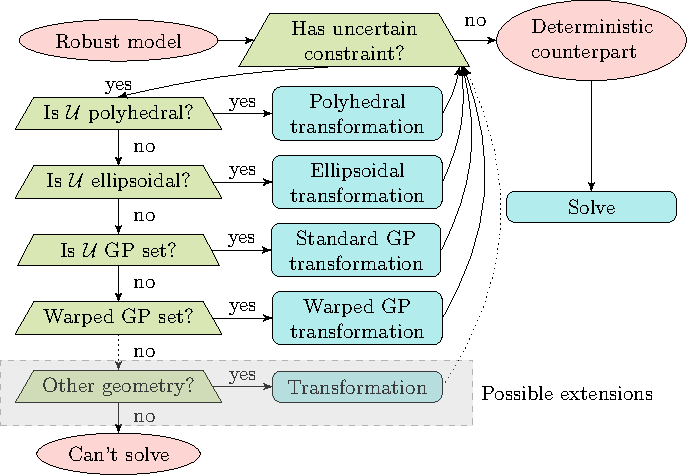
\includegraphics[width=0.7\linewidth]{img/reform}
    \tikzsetnextfilename{reform}
    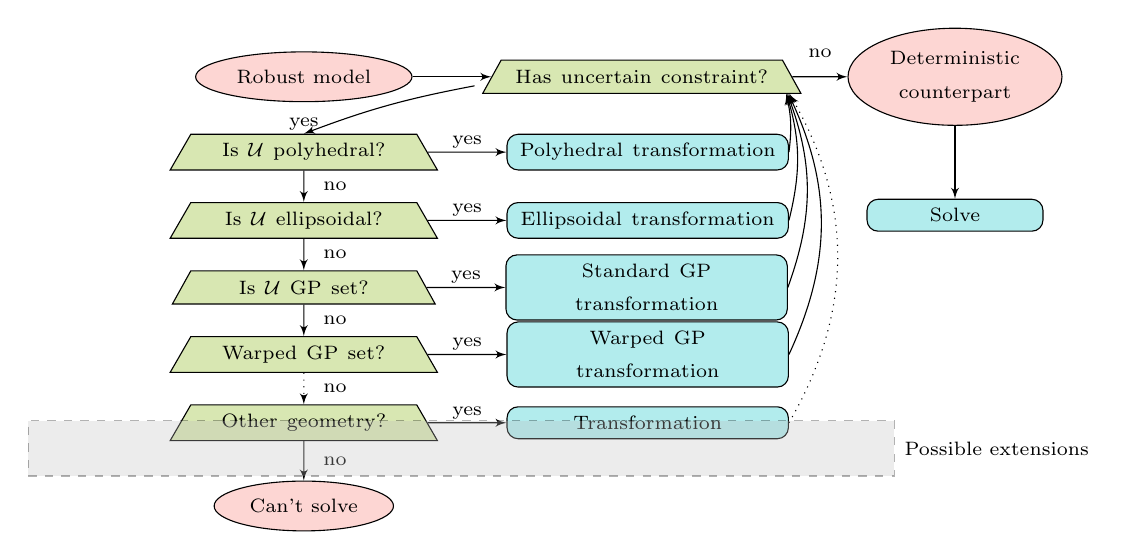
\begin{tikzpicture}
    \definecolor{00BFC4}{RGB}{0,191,196}
    \definecolor{C77CFF}{RGB}{199,124,255}
    \definecolor{F8766D}{RGB}{248,118,109}
    \definecolor{7CAE00}{RGB}{124,174,0}
    \tikzstyle{document} = [rectangle, draw,
                            fill=blue!30,
                            text width=4.7em,
                            text centered,
                            node distance=0.65cm,]
    \tikzstyle{block1} = [rectangle,
                          draw,
                          fill=00BFC4!30,
                          text centered,
                          rounded corners,
                          node distance=0.4cm,
                          minimum height=1.0em,
                          text width=9.5em]
    \tikzset{block/.style={trapezium,
                         draw,
                         trapezium stretches=true,
                         fill=7CAE00!30,
                         text centered,
                         node distance=0.4cm,
                         text width=7.5em,
                         minimum height=1.2em}}
    \tikzstyle{line} = [draw, -latex']
    \tikzstyle{cloud} = [draw,
                         ellipse,
                         fill=F8766D!30,
                         text centered,
                         node distance=0.2cm,
                         minimum height=1.8em]
    \tikzstyle{ioi} = [trapezium,draw,trapezium right angle=120,
                       rounded corners, fill=blue!60,
                       minimum height=2.2em]
    \tikzstyle{io} = [trapezium,draw,trapezium right angle=110,
                      rounded corners,fill=red!20,
                      minimum height=2.2em]   % the draw command here is used to draw the boundary of mentioned shape.  

    \node [cloud] (init) {\scriptsize Robust model};
    \node [block, right = 1cm of init, text width=9.5em](has_unc){\scriptsize Has uncertain constraint?};
    % Polyhedral
    \node [block, below = of init](is_poly){\scriptsize Is $\mathcal{U}$ polyhedral?};
    \node [block1, right =1cm of is_poly](poly){\scriptsize Polyhedral transformation};
    % Ellipsoidal
    \node [block, below = of is_poly](is_ell){\scriptsize Is $\mathcal{U}$ ellipsoidal?};
    \node [block1, right =1cm of is_ell](ell){\scriptsize Ellipsoidal transformation};
    % Standard GP
    \node [block, below = of is_ell](is_gp){\scriptsize Is $\mathcal{U}$ GP set?};
    \node [block1, right =1cm of is_gp](gp){\scriptsize Standard GP transformation};
    % Warped GP
    \node [block, below = of is_gp](is_wgp){\scriptsize Warped GP set?};
    \node [block1, right =1cm of is_wgp](wgp){\scriptsize Warped GP transformation};
    % Other geometry
    \node [block, below = of is_wgp](is_known){\scriptsize Other geometry?};
    \node [block1, right =1.0cm of is_known](trans){\scriptsize Transformation};
    % Cant solve
    \node [cloud, below = 0.5cm of is_known](cant_solve){\scriptsize Can't solve};
    \node [cloud,right = of has_unc,text width=4.80em,xshift=0.5cm] (counterpart) {\scriptsize Deterministic counterpart};
    \node [block1,below =0.925cm of counterpart,text width=2cm] (solve) {\scriptsize Solve};
    \node [below =-0.25cm of has_unc,xshift=1.8cm] (anchor_next) {};
    \node [below =-0.25cm of has_unc,xshift=-2.0cm] (anchor_is) {};

    % Arrows
    \path [line] (init) -- (has_unc);
    \path [line] (anchor_is) to [bend right=5] (is_poly.north)
        node[label={\scriptsize yes},yshift=-0.2cm] {};
    % Polyhedral
    \draw [line] (is_poly) -- (is_ell) node[midway,label=right:{\scriptsize no}] {};
    \path [line] (is_poly) -- (poly) node[midway,label=above:{\scriptsize yes},yshift=-0.2cm] {};
    \draw [line] (poly.east) to [bend right=10] (anchor_next) {};
    % Ellipsoidal
    \draw [line] (is_ell) -- (ell) node[midway,label=above:{\scriptsize yes},yshift=-0.2cm] {};
    \draw [line] (is_ell) -- (is_gp) node[midway,label=right:{\scriptsize no}] {};
    \draw [line] (ell.east) to [bend right=15] (anchor_next) {};
    % Standard GP
    \path [line] (is_gp) -- (gp) node[midway,label=above:{\scriptsize yes},yshift=-0.2cm] {};
    \draw [line] (is_gp) -- (is_wgp) node[midway,label=right:{\scriptsize no}] {};
    \draw [line] (gp.east) to [bend right=20] (anchor_next) {};
    % Warped GP
    \path [line] (is_wgp) -- (wgp) node[midway,label=above:{\scriptsize yes},yshift=-0.2cm] {};
    \draw [line,dotted] (is_wgp) -- (is_known) node[midway,label=right:{\scriptsize no}] {};
    \draw [line] (wgp.east) to [bend right=25] (anchor_next) {};
    % Extension
    \path [line] (is_known) -- (trans) node[midway,label=above:{\scriptsize yes},yshift=-0.2cm] {};
    \draw [line,dotted] (trans.east) to [bend right=30] (anchor_next);
    % Final
    \draw [line] (has_unc) -- (counterpart) node[midway,label=above:{\scriptsize no}] {};
    \draw [line] (counterpart) -- (solve);
    \path [line] (is_known) -- (cant_solve) node[midway,label=right:{\scriptsize no}] {};
    % Extension box
    \draw (2,-4.72) node [draw,
                          dashed,
                          minimum width=11cm,
                          minimum height=0.7cm,
                          fill=gray!50,
                          label=right:{\scriptsize Possible extensions},
                          opacity=0.3] {};
\end{tikzpicture}

\end{frame}

\begin{frame}{Solvers: cutting planes}
    \centering
    %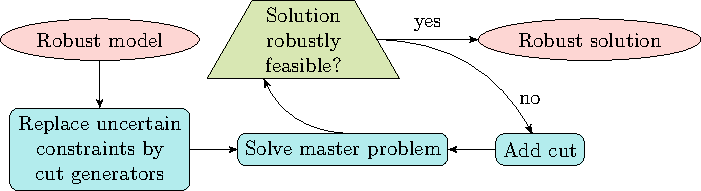
\includegraphics[width=0.7\linewidth]{img/cuts}
    \tikzsetnextfilename{cuts}
    \begin{tikzpicture}
    \definecolor{00BFC4}{RGB}{0,191,196}
    \definecolor{C77CFF}{RGB}{199,124,255}
    \definecolor{F8766D}{RGB}{248,118,109}
    \definecolor{7CAE00}{RGB}{124,174,0}
    \tikzstyle{document} = [rectangle, draw,
                            fill=blue!30,
                            text width=4.7em,
                            text centered,
                            node distance=1.0cm,]   
    \tikzstyle{block1} = [rectangle,
                          draw,
                          fill=00BFC4!30,
                          text centered,
                          rounded corners,
                          node distance=0.8cm,
                          minimum height=1.5em]
    \tikzstyle{block} = [trapezium,
                         draw,
                         fill=7CAE00!30,
                         text centered,
                         node distance=0.5cm,
                         text width=1.5cm,
                         %rounded corners,
                         minimum height=1.5em]
    \tikzstyle{line} = [draw, -latex']
    \tikzstyle{cloud} = [draw,
                         ellipse,
                         fill=F8766D!30,
                         node distance=0.2cm,
                         minimum height=2em]  
    \tikzstyle{ioi} = [trapezium,draw,trapezium right angle=120,
                       rounded corners, fill=blue!60,
                       minimum height=2.7em]  
    \tikzstyle{io} = [trapezium,draw,trapezium right angle=110,
                      rounded corners,fill=red!20,
                      node distance=0.2cm,
                      minimum height=2.9em]   % the draw command here is used to draw the boundary of mentioned shape.  

    \node [cloud] (init) {\small Robust model};
    \node [block1, below = of init,text width=8em](replace){\small Replace uncertain constraints by
        cut generators};
    \node [block1,right = of replace](master){\small Solve master problem};
    \node [block1,right = of master](cut){\small Add cut};
    \node [block,right = 1.22cm of init](feasible){\small Solution robustly feasible?};
    \node [cloud,right = of has_unc,] (sol) {\small Robust solution};

    \path [line] (init) -- (replace);
    \path [line] (replace) to (master);
    \path [line] (cut) to (master);
    \path [line] (master.north) to [bend left] (feasible.south west);
    \path [line] (feasible.east) to [bend left] node
        [midway,label=right:{no},xshift=0.6cm,yshift=-0.6cm] {} (cut);
    \path [line] (feasible) to node [midway,label=above:{yes},yshift=-0.1cm] {} (sol);

\end{tikzpicture}

\end{frame}


\begin{frame}{Extending ROmodel}
    ROmodel can be extended in a number of ways:
    \begin{enumerate}
        \item Implementing new library uncertainty set
        \item Adding new reformulations
    \end{enumerate}

    \visible<2->{
    \begin{exampleblock}{Gaussian process-based uncertainty sets}
        Gaussian processes are often used as surrogates for uncertain black-box
        constraints. We have developed reformulation approaches for
        chance constraints based on (warped) Gaussian processes [1].
    \end{exampleblock}
    \small
    [1] \cite{Wiebe2020}
}
\end{frame}

\begin{frame}[fragile]{Extending ROmodel: adding library sets}
    Class which collects relevant data:
\begin{lstlisting}[language=Python]
    class EllipsoidalSet(UncSet):
        '''
        Defines an ellipsoidal uncertainty set of shape:
            (param - mu)^T * A * (param - mu) <= 1
        '''
        def __init__(self, mean, cov, *args, **kwargs):
            self.mean = mean
            self.cov = cov
            super().__init__(*args, **kwargs)
\end{lstlisting}
    Make compatible with cutting planes:
\begin{lstlisting}[language=Python]
    def generate_cons_from_lib(self, param):
        raise NotImplementedError
\end{lstlisting}
\end{frame}

\begin{frame}[fragile]{Extending ROmodel: adding reformulations}
\begin{lstlisting}[language=Python]
    def _reformulate(self, c, param, uncset, counterpart):
        """
        Reformulate an uncertain constraint or objective
            c: Constraint or Objective
            param: UncParam
            uncset: UncSet
            counterpart: Block
        """
        return counterpart
\end{lstlisting}
Make compatible with generic uncertainty sets (\lstinline{UncSet}): \begin{lstlisting}[language=Python]
    def _check_applicability(self, uncset):
        """
        Returns `True` if the reformulation is applicable to `uncset`
        """
        return uncset.__class__ == GPSet
\end{lstlisting}
\end{frame}

\begin{frame}[fragile]{Extending ROmodel: Gaussian process-based sets}
    Train (warped) Gaussian process with GPy:
    \begin{lstlisting}[language=Python]
    import GPy
    # Set up kernel
    kernel = GPy.kern.RBF(input_dim=1)
    # Set up GP and train
    gp = GPy.models.WarpedGP(x, y, kernel=kernel, warping_terms=3)
    gp.optimize()
    \end{lstlisting}
    Use GPy model to construct uncertainty set:
    \begin{lstlisting}[language=Python]
    from romodel.uncset import WarpedGPSet
    m.z = pe.Var(range(3), within=pe.NonNegativeReals)
    # Set up GP-based uncertainty set
    m.uncset = WarpedGPSet(gp, m.z, 0.95)
    \end{lstlisting}
\end{frame}

\begin{frame}{Case studies}
    \begin{enumerate}
        \item Portolio optimization with uncertain returns [1],
        \item Knapsack problem with uncertain item weights,
        \item Pooling problem instance with uncertain product demands [2],
        \item Capacitated facility location problem with uncertain demand,
        \item Production planning problem with prices dependent on uncertain
            black-box function [3],
        \item Drill scheduling problem with uncertain degradation rate
            dependent on black-box function [3]
    \end{enumerate}
    \small
    [1] \cite{Bertsimas2004}, [2] \cite{adhya}, [3] \cite{Wiebe2020}
\end{frame}
\begin{frame}{Results: median times}
    \small
    \centering
\begin{tabular}{l l c c c}
                               &             & Reformulation    & Cuts & Overall \\ \hline
    \multirow{2}{*}{Knapsack}  & Polyhedral  & \phantom{601}54  & \phantom{40}272 & \phantom{753}85      \\
                               \cline{2-5}
                               & Ellipsoidal & \phantom{601}50  & \phantom{40}183 & \phantom{753}91      \\
%                                \cline{2-5}
%                                & Overall     & 68            & 252  & 84      \\
    \hline
    \multirow{2}{*}{Pooling}   & Polyhedral  & \phantom{601}74  & \phantom{40}329 & \phantom{75}173     \\
                               \cline{2-5}
                               & Ellipsoidal & \phantom{60}638  & \phantom{40}331 & \phantom{75}349    \\
%                                \cline{2-5}
%                                & Overall     & 123           & 487  & 483     \\
    \hline
    \multirow{2}{*}{Portfolio} & Polyhedral  & \phantom{601}50  & \phantom{40}276 & \phantom{75}126      \\
                               \cline{2-5}
                               & Ellipsoidal & \phantom{601}49  & \phantom{4}1659 & \phantom{75}129      \\
%                                \cline{2-5}
%                                & Overall     & 68            & 514  & 85      \\
    \hline
    \multirow{2}{*}{Facility}  & Polyhedral  & \phantom{60}261  & 13353           & \phantom{7}5588\\
                               \cline{2-5}
                               & Ellipsoidal & \phantom{601}--  & 31275           & 31275\\
    \hline
    \multirow{2}{*}{Planning}  & Standard    & \phantom{6}2776  & \phantom{400}NA & \phantom{7}2776\\
                               \cline{2-5}
                               & Warped      & \phantom{6}8536  & \phantom{400}NA & \phantom{7}8536\\
    \hline
    \multirow{2}{*}{Drilling}  & Standard    & 13646            & \phantom{400}NA & 13646 \\
                               \cline{2-5}
                               & Warped      & 75325            & \phantom{400}NA & 75325\\
    \hline
                        Overall&             & \phantom{601}74  & \phantom{40}330 & \phantom{75}271     \\
    \hline
\end{tabular}
\end{frame}

\begin{frame}{Results: price of robustness}
    \centering
    % 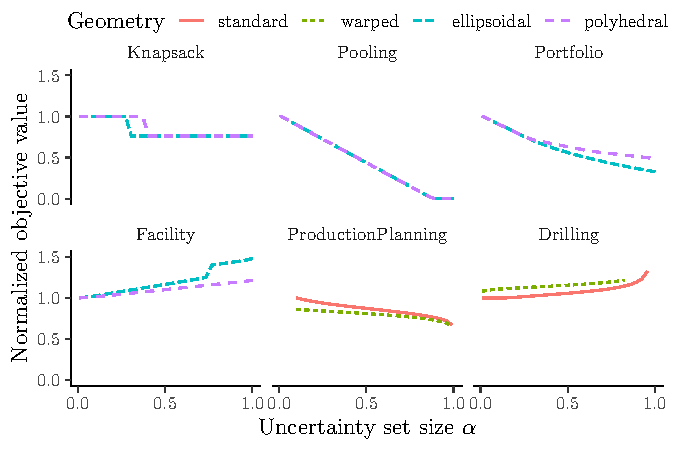
\includegraphics[width=0.8\textwidth]{img/results.pdf}
    \tikzsetnextfilename{results}
    % Created by tikzDevice version 0.12.3.1 on 2021-03-23 11:05:25
% !TEX encoding = UTF-8 Unicode
\begin{tikzpicture}[x=1pt,y=1pt]
\InputIfFileExists{/home/johannes/papers/romodel/journal/img/results_colors.tex}{}{}
\definecolor{mbg}{RGB}{250,250,250}
\path[use as bounding box,fill=transparent,fill opacity=1.00] (0,0) rectangle (325.21,216.81);
\begin{scope}
\path[clip] (  0.00,  0.00) rectangle (325.21,216.81);

\path[draw=transparent,line width= 0.6pt,line join=round,line cap=round,fill=mbg] (  0.00,  0.00) rectangle (325.21,216.81);
\end{scope}
\begin{scope}
\path[clip] ( 34.16,118.13) rectangle (125.68,183.51);

\path[fill=mbg] ( 34.16,118.13) rectangle (125.68,183.51);

\path[draw=00BFC4,line width= 1.1pt,dash pattern=on 4pt off 2pt ,line join=round] ( 38.32,160.73) --
	( 38.32,160.73) --
	( 38.32,160.73) --
	( 38.32,160.73) --
	( 41.09,160.73) --
	( 41.09,160.73) --
	( 41.09,160.73) --
	( 41.09,160.73) --
	( 43.86,160.73) --
	( 43.86,160.73) --
	( 43.86,160.73) --
	( 43.86,160.73) --
	( 46.64,160.73) --
	( 46.64,160.73) --
	( 46.64,160.73) --
	( 46.64,160.73) --
	( 49.41,160.73) --
	( 49.41,160.73) --
	( 49.41,160.73) --
	( 49.41,160.73) --
	( 52.18,160.73) --
	( 52.18,160.73) --
	( 52.18,160.73) --
	( 52.18,160.73) --
	( 54.96,160.73) --
	( 54.96,160.73) --
	( 54.96,160.73) --
	( 54.96,160.73) --
	( 57.73,160.73) --
	( 57.73,160.73) --
	( 57.73,160.73) --
	( 57.73,160.73) --
	( 60.50,160.73) --
	( 60.50,160.73) --
	( 60.50,160.73) --
	( 60.50,160.73) --
	( 63.28,151.22) --
	( 63.28,151.22) --
	( 63.28,151.22) --
	( 63.28,151.22) --
	( 66.05,151.22) --
	( 66.05,151.22) --
	( 66.05,151.22) --
	( 66.05,151.22) --
	( 68.82,151.22) --
	( 68.82,151.22) --
	( 68.82,151.22) --
	( 68.82,151.22) --
	( 71.60,151.22) --
	( 71.60,151.22) --
	( 71.60,151.22) --
	( 71.60,151.22) --
	( 74.37,151.22) --
	( 74.37,151.22) --
	( 74.37,151.22) --
	( 74.37,151.22) --
	( 77.14,151.22) --
	( 77.14,151.22) --
	( 77.14,151.22) --
	( 77.14,151.22) --
	( 79.92,151.22) --
	( 79.92,151.22) --
	( 79.92,151.22) --
	( 79.92,151.22) --
	( 82.69,151.22) --
	( 82.69,151.22) --
	( 82.69,151.22) --
	( 82.69,151.22) --
	( 85.46,151.22) --
	( 85.46,151.22) --
	( 85.46,151.22) --
	( 85.46,151.22) --
	( 88.24,151.22) --
	( 88.24,151.22) --
	( 88.24,151.22) --
	( 88.24,151.22) --
	( 91.01,151.22) --
	( 91.01,151.22) --
	( 91.01,151.22) --
	( 91.01,151.22) --
	( 93.78,151.22) --
	( 93.78,151.22) --
	( 93.78,151.22) --
	( 93.78,151.22) --
	( 96.56,151.22) --
	( 96.56,151.22) --
	( 96.56,151.22) --
	( 96.56,151.22) --
	( 99.33,151.22) --
	( 99.33,151.22) --
	( 99.33,151.22) --
	( 99.33,151.22) --
	(102.10,151.22) --
	(102.10,151.22) --
	(102.10,151.22) --
	(102.10,151.22) --
	(104.88,151.22) --
	(104.88,151.22) --
	(104.88,151.22) --
	(104.88,151.22) --
	(107.65,151.22) --
	(107.65,151.22) --
	(107.65,151.22) --
	(107.65,151.22) --
	(110.42,151.22) --
	(110.42,151.22) --
	(110.42,151.22) --
	(110.42,151.22) --
	(113.20,151.22) --
	(113.20,151.22) --
	(113.20,151.22) --
	(113.20,151.22) --
	(115.97,151.22) --
	(115.97,151.22) --
	(115.97,151.22) --
	(115.97,151.22) --
	(118.74,151.22) --
	(118.74,151.22) --
	(118.74,151.22) --
	(118.74,151.22) --
	(121.52,151.22) --
	(121.52,151.22) --
	(121.52,151.22) --
	(121.52,151.22);

\path[draw=C77CFF,line width= 1.1pt,dash pattern=on 4pt off 4pt ,line join=round] ( 38.32,160.73) --
	( 38.32,160.73) --
	( 38.32,160.73) --
	( 38.32,160.73) --
	( 41.09,160.73) --
	( 41.09,160.73) --
	( 41.09,160.73) --
	( 41.09,160.73) --
	( 43.86,160.73) --
	( 43.86,160.73) --
	( 43.86,160.73) --
	( 43.86,160.73) --
	( 46.64,160.73) --
	( 46.64,160.73) --
	( 46.64,160.73) --
	( 46.64,160.73) --
	( 49.41,160.73) --
	( 49.41,160.73) --
	( 49.41,160.73) --
	( 49.41,160.73) --
	( 52.18,160.73) --
	( 52.18,160.73) --
	( 52.18,160.73) --
	( 52.18,160.73) --
	( 54.96,160.73) --
	( 54.96,160.73) --
	( 54.96,160.73) --
	( 54.96,160.73) --
	( 57.73,160.73) --
	( 57.73,160.73) --
	( 57.73,160.73) --
	( 57.73,160.73) --
	( 60.50,160.73) --
	( 60.50,160.73) --
	( 60.50,160.73) --
	( 60.50,160.73) --
	( 63.28,160.73) --
	( 63.28,160.73) --
	( 63.28,160.73) --
	( 63.28,160.73) --
	( 66.05,160.73) --
	( 66.05,160.73) --
	( 66.05,160.73) --
	( 66.05,160.73) --
	( 68.82,160.73) --
	( 68.82,160.73) --
	( 68.82,160.73) --
	( 68.82,160.73) --
	( 71.60,151.22) --
	( 71.60,151.22) --
	( 71.60,151.22) --
	( 71.60,151.22) --
	( 74.37,151.22) --
	( 74.37,151.22) --
	( 74.37,151.22) --
	( 74.37,151.22) --
	( 77.14,151.22) --
	( 77.14,151.22) --
	( 77.14,151.22) --
	( 77.14,151.22) --
	( 79.92,151.22) --
	( 79.92,151.22) --
	( 79.92,151.22) --
	( 79.92,151.22) --
	( 82.69,151.22) --
	( 82.69,151.22) --
	( 82.69,151.22) --
	( 82.69,151.22) --
	( 85.46,151.22) --
	( 85.46,151.22) --
	( 85.46,151.22) --
	( 85.46,151.22) --
	( 88.24,151.22) --
	( 88.24,151.22) --
	( 88.24,151.22) --
	( 88.24,151.22) --
	( 91.01,151.22) --
	( 91.01,151.22) --
	( 91.01,151.22) --
	( 91.01,151.22) --
	( 93.78,151.22) --
	( 93.78,151.22) --
	( 93.78,151.22) --
	( 93.78,151.22) --
	( 96.56,151.22) --
	( 96.56,151.22) --
	( 96.56,151.22) --
	( 96.56,151.22) --
	( 99.33,151.22) --
	( 99.33,151.22) --
	( 99.33,151.22) --
	( 99.33,151.22) --
	(102.10,151.22) --
	(102.10,151.22) --
	(102.10,151.22) --
	(102.10,151.22) --
	(104.88,151.22) --
	(104.88,151.22) --
	(104.88,151.22) --
	(104.88,151.22) --
	(107.65,151.22) --
	(107.65,151.22) --
	(107.65,151.22) --
	(107.65,151.22) --
	(110.42,151.22) --
	(110.42,151.22) --
	(110.42,151.22) --
	(110.42,151.22) --
	(113.20,151.22) --
	(113.20,151.22) --
	(113.20,151.22) --
	(113.20,151.22) --
	(115.97,151.22) --
	(115.97,151.22) --
	(115.97,151.22) --
	(115.97,151.22) --
	(118.74,151.22) --
	(118.74,151.22) --
	(118.74,151.22) --
	(118.74,151.22) --
	(121.52,151.22) --
	(121.52,151.22) --
	(121.52,151.22) --
	(121.52,151.22);
\end{scope}
\begin{scope}
\path[clip] ( 34.16, 30.69) rectangle (125.68, 96.06);

\path[fill=mbg] ( 34.16, 30.69) rectangle (125.68, 96.06);

\path[draw=00BFC4,line width= 1.1pt,dash pattern=on 4pt off 2pt ,line join=round] ( 38.32, 73.31) --
	( 38.32, 73.31) --
	( 41.09, 73.61) --
	( 41.09, 73.61) --
	( 43.86, 73.96) --
	( 43.86, 73.96) --
	( 46.64, 74.39) --
	( 46.64, 74.39) --
	( 49.41, 74.83) --
	( 49.41, 74.83) --
	( 52.18, 75.29) --
	( 52.18, 75.29) --
	( 54.96, 75.75) --
	( 54.96, 75.75) --
	( 57.73, 76.20) --
	( 57.73, 76.20) --
	( 60.50, 76.66) --
	( 60.50, 76.66) --
	( 63.28, 77.12) --
	( 63.28, 77.12) --
	( 66.05, 77.58) --
	( 66.05, 77.58) --
	( 68.82, 78.04) --
	( 68.82, 78.04) --
	( 71.60, 78.50) --
	( 71.60, 78.50) --
	( 74.37, 78.95) --
	( 74.37, 78.95) --
	( 77.14, 79.41) --
	( 77.14, 79.41) --
	( 79.92, 79.87) --
	( 79.92, 79.87) --
	( 82.69, 80.33) --
	( 82.69, 80.33) --
	( 85.46, 80.79) --
	( 85.46, 80.79) --
	( 88.24, 81.25) --
	( 88.24, 81.25) --
	( 91.01, 81.70) --
	( 91.01, 81.70) --
	( 93.78, 82.16) --
	( 93.78, 82.16) --
	( 96.56, 82.63) --
	( 96.56, 82.63) --
	( 99.33, 83.25) --
	( 99.33, 83.25) --
	(102.10, 89.12) --
	(102.10, 89.12) --
	(104.88, 89.50) --
	(104.88, 89.50) --
	(107.65, 89.88) --
	(107.65, 89.88) --
	(110.42, 90.27) --
	(110.42, 90.27) --
	(113.20, 90.67) --
	(113.20, 90.67) --
	(115.97, 91.09) --
	(115.97, 91.09) --
	(118.74, 91.55) --
	(118.74, 91.55) --
	(121.52, 92.24) --
	(121.52, 92.24);

\path[draw=C77CFF,line width= 1.1pt,dash pattern=on 4pt off 4pt ,line join=round] ( 38.32, 73.28) --
	( 38.32, 73.28) --
	( 38.32, 73.28) --
	( 38.32, 73.28) --
	( 41.09, 73.47) --
	( 41.09, 73.47) --
	( 41.09, 73.47) --
	( 41.09, 73.47) --
	( 43.86, 73.65) --
	( 43.86, 73.65) --
	( 43.86, 73.65) --
	( 43.86, 73.65) --
	( 46.64, 73.84) --
	( 46.64, 73.84) --
	( 46.64, 73.84) --
	( 46.64, 73.84) --
	( 49.41, 74.11) --
	( 49.41, 74.11) --
	( 49.41, 74.11) --
	( 49.41, 74.11) --
	( 52.18, 74.40) --
	( 52.18, 74.40) --
	( 52.18, 74.40) --
	( 52.18, 74.40) --
	( 54.96, 74.69) --
	( 54.96, 74.69) --
	( 54.96, 74.69) --
	( 54.96, 74.69) --
	( 57.73, 74.98) --
	( 57.73, 74.98) --
	( 57.73, 74.98) --
	( 57.73, 74.98) --
	( 60.50, 75.27) --
	( 60.50, 75.27) --
	( 60.50, 75.27) --
	( 60.50, 75.27) --
	( 63.28, 75.56) --
	( 63.28, 75.56) --
	( 63.28, 75.56) --
	( 63.28, 75.56) --
	( 66.05, 75.85) --
	( 66.05, 75.85) --
	( 66.05, 75.85) --
	( 66.05, 75.85) --
	( 68.82, 76.14) --
	( 68.82, 76.14) --
	( 68.82, 76.14) --
	( 68.82, 76.14) --
	( 71.60, 76.43) --
	( 71.60, 76.43) --
	( 71.60, 76.43) --
	( 71.60, 76.43) --
	( 74.37, 76.72) --
	( 74.37, 76.72) --
	( 74.37, 76.72) --
	( 74.37, 76.72) --
	( 77.14, 77.01) --
	( 77.14, 77.01) --
	( 77.14, 77.01) --
	( 77.14, 77.01) --
	( 79.92, 77.30) --
	( 79.92, 77.30) --
	( 79.92, 77.30) --
	( 79.92, 77.30) --
	( 82.69, 77.60) --
	( 82.69, 77.60) --
	( 82.69, 77.60) --
	( 82.69, 77.60) --
	( 85.46, 77.89) --
	( 85.46, 77.89) --
	( 85.46, 77.89) --
	( 85.46, 77.89) --
	( 88.24, 78.18) --
	( 88.24, 78.18) --
	( 88.24, 78.18) --
	( 88.24, 78.18) --
	( 91.01, 78.47) --
	( 91.01, 78.47) --
	( 91.01, 78.47) --
	( 91.01, 78.47) --
	( 93.78, 78.76) --
	( 93.78, 78.76) --
	( 93.78, 78.76) --
	( 93.78, 78.76) --
	( 96.56, 79.05) --
	( 96.56, 79.05) --
	( 96.56, 79.05) --
	( 96.56, 79.05) --
	( 99.33, 79.34) --
	( 99.33, 79.34) --
	( 99.33, 79.34) --
	( 99.33, 79.34) --
	(102.10, 79.63) --
	(102.10, 79.63) --
	(102.10, 79.63) --
	(102.10, 79.63) --
	(104.88, 79.92) --
	(104.88, 79.92) --
	(104.88, 79.92) --
	(104.88, 79.92) --
	(107.65, 80.21) --
	(107.65, 80.21) --
	(107.65, 80.21) --
	(107.65, 80.21) --
	(110.42, 80.50) --
	(110.42, 80.50) --
	(110.42, 80.50) --
	(110.42, 80.50) --
	(113.20, 80.79) --
	(113.20, 80.79) --
	(113.20, 80.79) --
	(113.20, 80.79) --
	(115.97, 81.08) --
	(115.97, 81.08) --
	(115.97, 81.08) --
	(115.97, 81.08) --
	(118.74, 81.37) --
	(118.74, 81.37) --
	(118.74, 81.37) --
	(118.74, 81.37) --
	(121.52, 81.66) --
	(121.52, 81.66) --
	(121.52, 81.66) --
	(121.52, 81.66);
\end{scope}
\begin{scope}
\path[clip] (131.18,118.13) rectangle (222.70,183.51);

\path[fill=mbg] (131.18,118.13) rectangle (222.70,183.51);

\path[draw=00BFC4,line width= 1.1pt,dash pattern=on 4pt off 2pt ,line join=round] (135.34,160.63) --
	(135.34,160.63) --
	(135.34,160.73) --
	(135.34,160.73) --
	(138.11,159.23) --
	(138.11,159.23) --
	(138.11,159.23) --
	(138.11,159.23) --
	(140.88,157.72) --
	(140.88,157.72) --
	(140.88,157.72) --
	(140.88,157.72) --
	(143.66,156.22) --
	(143.66,156.22) --
	(143.66,156.22) --
	(143.66,156.22) --
	(146.43,154.72) --
	(146.43,154.72) --
	(146.43,154.72) --
	(146.43,154.72) --
	(149.20,153.21) --
	(149.20,153.21) --
	(149.20,153.21) --
	(149.20,153.21) --
	(151.98,151.71) --
	(151.98,151.71) --
	(151.98,151.71) --
	(151.98,151.71) --
	(154.75,150.21) --
	(154.75,150.21) --
	(154.75,150.21) --
	(154.75,150.21) --
	(157.52,148.70) --
	(157.52,148.70) --
	(157.52,148.70) --
	(157.52,148.70) --
	(160.30,147.20) --
	(160.30,147.20) --
	(160.30,147.20) --
	(160.30,147.20) --
	(163.07,145.70) --
	(163.07,145.70) --
	(163.07,145.70) --
	(163.07,145.70) --
	(165.84,144.20) --
	(165.84,144.20) --
	(165.84,144.20) --
	(165.84,144.20) --
	(168.62,142.69) --
	(168.62,142.69) --
	(168.62,142.69) --
	(168.62,142.69) --
	(171.39,141.19) --
	(171.39,141.19) --
	(171.39,141.19) --
	(171.39,141.19) --
	(174.16,139.69) --
	(174.16,139.69) --
	(174.16,139.69) --
	(174.16,139.69) --
	(176.94,138.18) --
	(176.94,138.18) --
	(176.94,138.18) --
	(176.94,138.18) --
	(179.71,136.68) --
	(179.71,136.68) --
	(179.71,136.68) --
	(179.71,136.68) --
	(182.48,135.18) --
	(182.48,135.18) --
	(182.48,135.18) --
	(182.48,135.18) --
	(185.26,133.68) --
	(185.26,133.68) --
	(185.26,133.68) --
	(185.26,133.68) --
	(188.03,132.17) --
	(188.03,132.17) --
	(188.03,132.17) --
	(188.03,132.17) --
	(190.80,130.67) --
	(190.80,130.67) --
	(190.80,130.67) --
	(190.80,130.67) --
	(193.58,129.17) --
	(193.58,129.17) --
	(193.58,129.17) --
	(193.58,129.17) --
	(196.35,127.66) --
	(196.35,127.66) --
	(196.35,127.66) --
	(196.35,127.66) --
	(199.12,126.16) --
	(199.12,126.16) --
	(199.12,126.16) --
	(199.12,126.16) --
	(201.90,124.66) --
	(201.90,124.66) --
	(201.90,124.66) --
	(201.90,124.66) --
	(204.67,123.16) --
	(204.67,123.16) --
	(204.67,123.16) --
	(204.67,123.16) --
	(207.44,121.65) --
	(207.44,121.65) --
	(207.44,121.65) --
	(207.44,121.65) --
	(210.22,121.11) --
	(210.22,121.11) --
	(210.22,121.11) --
	(210.22,121.11) --
	(212.99,121.11) --
	(212.99,121.11) --
	(212.99,121.11) --
	(212.99,121.11) --
	(215.76,121.11) --
	(215.76,121.11) --
	(215.76,121.11) --
	(215.76,121.11) --
	(218.54,121.11) --
	(218.54,121.11) --
	(218.54,121.11) --
	(218.54,121.11);

\path[draw=C77CFF,line width= 1.1pt,dash pattern=on 4pt off 4pt ,line join=round] (135.34,160.63) --
	(135.34,160.63) --
	(135.34,160.73) --
	(135.34,160.73) --
	(138.11,159.23) --
	(138.11,159.23) --
	(138.11,159.23) --
	(138.11,159.23) --
	(140.88,157.72) --
	(140.88,157.72) --
	(140.88,157.72) --
	(140.88,157.72) --
	(143.66,156.22) --
	(143.66,156.22) --
	(143.66,156.22) --
	(143.66,156.22) --
	(146.43,154.72) --
	(146.43,154.72) --
	(146.43,154.72) --
	(146.43,154.72) --
	(149.20,153.21) --
	(149.20,153.21) --
	(149.20,153.21) --
	(149.20,153.21) --
	(151.98,151.71) --
	(151.98,151.71) --
	(151.98,151.71) --
	(151.98,151.71) --
	(154.75,150.21) --
	(154.75,150.21) --
	(154.75,150.21) --
	(154.75,150.21) --
	(157.52,148.70) --
	(157.52,148.70) --
	(157.52,148.70) --
	(157.52,148.70) --
	(160.30,147.20) --
	(160.30,147.20) --
	(160.30,147.20) --
	(160.30,147.20) --
	(163.07,145.70) --
	(163.07,145.70) --
	(163.07,145.70) --
	(163.07,145.70) --
	(165.84,144.20) --
	(165.84,144.20) --
	(165.84,144.20) --
	(165.84,144.20) --
	(168.62,142.69) --
	(168.62,142.69) --
	(168.62,142.69) --
	(168.62,142.69) --
	(171.39,141.19) --
	(171.39,141.19) --
	(171.39,141.19) --
	(171.39,141.19) --
	(174.16,139.69) --
	(174.16,139.69) --
	(174.16,139.69) --
	(174.16,139.69) --
	(176.94,138.18) --
	(176.94,138.18) --
	(176.94,138.18) --
	(176.94,138.18) --
	(179.71,136.68) --
	(179.71,136.68) --
	(179.71,136.68) --
	(179.71,136.68) --
	(182.48,135.18) --
	(182.48,135.18) --
	(182.48,135.18) --
	(182.48,135.18) --
	(185.26,133.68) --
	(185.26,133.68) --
	(185.26,133.68) --
	(185.26,133.68) --
	(188.03,132.17) --
	(188.03,132.17) --
	(188.03,132.17) --
	(188.03,132.17) --
	(190.80,130.67) --
	(190.80,130.67) --
	(190.80,130.67) --
	(190.80,130.67) --
	(193.58,129.17) --
	(193.58,129.17) --
	(193.58,129.17) --
	(193.58,129.17) --
	(196.35,127.66) --
	(196.35,127.66) --
	(196.35,127.66) --
	(196.35,127.66) --
	(199.12,126.16) --
	(199.12,126.16) --
	(199.12,126.16) --
	(199.12,126.16) --
	(201.90,124.66) --
	(201.90,124.66) --
	(201.90,124.66) --
	(201.90,124.66) --
	(204.67,123.16) --
	(204.67,123.16) --
	(204.67,123.16) --
	(204.67,123.16) --
	(207.44,121.65) --
	(207.44,121.65) --
	(207.44,121.65) --
	(207.44,121.65) --
	(210.22,121.11) --
	(210.22,121.11) --
	(210.22,121.11) --
	(210.22,121.11) --
	(212.99,121.11) --
	(212.99,121.11) --
	(212.99,121.11) --
	(212.99,121.11) --
	(215.76,121.11) --
	(215.76,121.11) --
	(215.76,121.11) --
	(215.76,121.11) --
	(218.54,121.11) --
	(218.54,121.11) --
	(218.54,121.11) --
	(218.54,121.11);
\end{scope}
\begin{scope}
\path[clip] (131.18, 30.69) rectangle (222.70, 96.06);

\path[fill=mbg] (131.18, 30.69) rectangle (222.70, 96.06);

\path[draw=F8766D,line width= 1.1pt,line join=round] (142.90, 73.28) --
	(145.39, 72.64) --
	(147.89, 72.11) --
	(150.38, 71.64) --
	(152.87, 71.22) --
	(155.37, 70.84) --
	(157.86, 70.48) --
	(160.35, 70.14) --
	(162.84, 69.82) --
	(165.34, 69.51) --
	(167.83, 69.22) --
	(170.32, 68.93) --
	(172.82, 68.64) --
	(175.31, 68.36) --
	(177.80, 68.08) --
	(180.30, 67.81) --
	(182.79, 67.53) --
	(185.28, 67.25) --
	(187.78, 66.96) --
	(190.27, 66.67) --
	(192.76, 66.38) --
	(195.26, 66.07) --
	(197.75, 65.74) --
	(200.24, 65.40) --
	(202.74, 65.03) --
	(205.23, 64.63) --
	(207.72, 64.18) --
	(210.22, 63.65) --
	(212.71, 63.01) --
	(215.20, 62.11) --
	(217.69, 60.28);

\path[draw=7CAE00,line width= 1.1pt,dash pattern=on 2pt off 2pt ,line join=round] (142.90, 67.71) --
	(145.39, 67.57) --
	(147.89, 67.43) --
	(150.38, 67.29) --
	(152.87, 67.15) --
	(155.37, 67.01) --
	(157.86, 66.86) --
	(160.35, 66.72) --
	(162.84, 66.57) --
	(165.34, 66.42) --
	(167.83, 66.27) --
	(170.32, 66.12) --
	(172.82, 65.96) --
	(175.31, 65.80) --
	(177.80, 65.64) --
	(180.30, 65.46) --
	(182.79, 65.29) --
	(185.28, 65.11) --
	(187.78, 64.92) --
	(190.27, 64.72) --
	(192.76, 64.51) --
	(195.26, 64.28) --
	(197.75, 64.04) --
	(200.24, 63.79) --
	(202.74, 63.50) --
	(205.23, 63.19) --
	(207.72, 62.83) --
	(210.22, 62.40) --
	(212.71, 61.85) --
	(215.20, 61.08) --
	(217.69, 59.47);
\end{scope}
\begin{scope}
\path[clip] (228.20,118.13) rectangle (319.71,183.51);

\path[fill=mbg] (228.20,118.13) rectangle (319.71,183.51);

\path[draw=00BFC4,line width= 1.1pt,dash pattern=on 4pt off 2pt ,line join=round] (232.36,160.73) --
	(232.36,160.73) --
	(232.36,160.73) --
	(232.36,160.73) --
	(235.13,159.41) --
	(235.13,159.41) --
	(235.13,159.41) --
	(235.13,159.41) --
	(237.90,158.09) --
	(237.90,158.09) --
	(237.90,158.09) --
	(237.90,158.09) --
	(240.68,156.77) --
	(240.68,156.77) --
	(240.68,156.77) --
	(240.68,156.77) --
	(243.45,155.45) --
	(243.45,155.45) --
	(243.45,155.45) --
	(243.45,155.45) --
	(246.22,154.12) --
	(246.22,154.12) --
	(246.22,154.12) --
	(246.22,154.12) --
	(249.00,152.80) --
	(249.00,152.80) --
	(249.00,152.80) --
	(249.00,152.80) --
	(251.77,151.48) --
	(251.77,151.48) --
	(251.77,151.48) --
	(251.77,151.48) --
	(254.54,150.16) --
	(254.54,150.16) --
	(254.54,150.16) --
	(254.54,150.16) --
	(257.32,148.89) --
	(257.32,148.89) --
	(257.32,148.89) --
	(257.32,148.89) --
	(260.09,147.79) --
	(260.09,147.79) --
	(260.09,147.79) --
	(260.09,147.79) --
	(262.86,146.77) --
	(262.86,146.77) --
	(262.86,146.77) --
	(262.86,146.77) --
	(265.64,145.81) --
	(265.64,145.81) --
	(265.64,145.81) --
	(265.64,145.81) --
	(268.41,144.89) --
	(268.41,144.89) --
	(268.41,144.89) --
	(268.41,144.89) --
	(271.18,144.00) --
	(271.18,144.00) --
	(271.18,144.00) --
	(271.18,144.00) --
	(273.96,143.16) --
	(273.96,143.16) --
	(273.96,143.16) --
	(273.96,143.16) --
	(276.73,142.39) --
	(276.73,142.39) --
	(276.73,142.39) --
	(276.73,142.39) --
	(279.50,141.66) --
	(279.50,141.66) --
	(279.50,141.66) --
	(279.50,141.66) --
	(282.28,140.96) --
	(282.28,140.96) --
	(282.28,140.96) --
	(282.28,140.96) --
	(285.05,140.28) --
	(285.05,140.28) --
	(285.05,140.28) --
	(285.05,140.28) --
	(287.82,139.63) --
	(287.82,139.63) --
	(287.82,139.62) --
	(287.82,139.62) --
	(290.60,138.98) --
	(290.60,138.98) --
	(290.60,138.98) --
	(290.60,138.98) --
	(293.37,138.35) --
	(293.37,138.35) --
	(293.37,138.35) --
	(293.37,138.35) --
	(296.14,137.74) --
	(296.14,137.74) --
	(296.14,137.74) --
	(296.14,137.74) --
	(298.92,137.17) --
	(298.92,137.17) --
	(298.92,137.17) --
	(298.92,137.17) --
	(301.69,136.62) --
	(301.69,136.62) --
	(301.69,136.61) --
	(301.69,136.61) --
	(304.46,136.08) --
	(304.46,136.08) --
	(304.46,136.08) --
	(304.46,136.08) --
	(307.24,135.57) --
	(307.24,135.57) --
	(307.24,135.57) --
	(307.24,135.57) --
	(310.01,135.07) --
	(310.01,135.07) --
	(310.01,135.07) --
	(310.01,135.07) --
	(312.78,134.57) --
	(312.78,134.57) --
	(312.78,134.57) --
	(312.78,134.57) --
	(315.56,134.09) --
	(315.56,134.09) --
	(315.56,134.09) --
	(315.56,134.09);

\path[draw=C77CFF,line width= 1.1pt,dash pattern=on 4pt off 4pt ,line join=round] (232.36,160.73) --
	(232.36,160.73) --
	(232.36,160.73) --
	(232.36,160.73) --
	(235.13,159.41) --
	(235.13,159.41) --
	(235.13,159.41) --
	(235.13,159.41) --
	(237.90,158.09) --
	(237.90,158.09) --
	(237.90,158.09) --
	(237.90,158.09) --
	(240.68,156.77) --
	(240.68,156.77) --
	(240.68,156.77) --
	(240.68,156.77) --
	(243.45,155.45) --
	(243.45,155.45) --
	(243.45,155.45) --
	(243.45,155.45) --
	(246.22,154.12) --
	(246.22,154.12) --
	(246.22,154.12) --
	(246.22,154.12) --
	(249.00,152.80) --
	(249.00,152.80) --
	(249.00,152.80) --
	(249.00,152.80) --
	(251.77,151.48) --
	(251.77,151.48) --
	(251.77,151.48) --
	(251.77,151.48) --
	(254.54,150.16) --
	(254.54,150.16) --
	(254.54,150.16) --
	(254.54,150.16) --
	(257.32,149.34) --
	(257.32,149.34) --
	(257.32,149.34) --
	(257.32,149.34) --
	(260.09,148.79) --
	(260.09,148.79) --
	(260.09,148.79) --
	(260.09,148.79) --
	(262.86,148.24) --
	(262.86,148.24) --
	(262.86,148.24) --
	(262.86,148.24) --
	(265.64,147.69) --
	(265.64,147.69) --
	(265.64,147.69) --
	(265.64,147.69) --
	(268.41,147.14) --
	(268.41,147.14) --
	(268.41,147.14) --
	(268.41,147.14) --
	(271.18,146.59) --
	(271.18,146.59) --
	(271.18,146.59) --
	(271.18,146.59) --
	(273.96,146.04) --
	(273.96,146.04) --
	(273.96,146.04) --
	(273.96,146.04) --
	(276.73,145.49) --
	(276.73,145.49) --
	(276.73,145.49) --
	(276.73,145.49) --
	(279.50,144.94) --
	(279.50,144.94) --
	(279.50,144.94) --
	(279.50,144.94) --
	(282.28,144.39) --
	(282.28,144.39) --
	(282.28,144.39) --
	(282.28,144.39) --
	(285.05,143.89) --
	(285.05,143.89) --
	(285.05,143.89) --
	(285.05,143.89) --
	(287.82,143.58) --
	(287.82,143.58) --
	(287.82,143.58) --
	(287.82,143.58) --
	(290.60,143.26) --
	(290.60,143.26) --
	(290.60,143.26) --
	(290.60,143.26) --
	(293.37,142.94) --
	(293.37,142.94) --
	(293.37,142.94) --
	(293.37,142.94) --
	(296.14,142.62) --
	(296.14,142.62) --
	(296.14,142.62) --
	(296.14,142.62) --
	(298.92,142.30) --
	(298.92,142.30) --
	(298.92,142.30) --
	(298.92,142.30) --
	(301.69,141.98) --
	(301.69,141.98) --
	(301.69,141.98) --
	(301.69,141.98) --
	(304.46,141.67) --
	(304.46,141.67) --
	(304.46,141.67) --
	(304.46,141.67) --
	(307.24,141.35) --
	(307.24,141.35) --
	(307.24,141.35) --
	(307.24,141.35) --
	(310.01,141.03) --
	(310.01,141.03) --
	(310.01,141.03) --
	(310.01,141.03) --
	(312.78,140.71) --
	(312.78,140.71) --
	(312.78,140.71) --
	(312.78,140.71) --
	(315.56,140.39) --
	(315.56,140.39) --
	(315.56,140.39) --
	(315.56,140.39);
\end{scope}
\begin{scope}
\path[clip] (228.20, 30.69) rectangle (319.71, 96.06);

\path[fill=mbg] (228.20, 30.69) rectangle (319.71, 96.06);

\path[draw=F8766D,line width= 1.1pt,line join=round] (232.36, 73.28) --
	(235.10, 73.28) --
	(237.85, 73.28) --
	(240.59, 73.28) --
	(243.34, 73.28) --
	(246.08, 73.36) --
	(248.83, 73.60) --
	(251.57, 73.82) --
	(254.32, 74.03) --
	(257.06, 74.24) --
	(259.81, 74.45) --
	(262.55, 74.65) --
	(265.30, 74.86) --
	(268.04, 75.07) --
	(270.79, 75.29) --
	(273.53, 75.51) --
	(276.28, 75.74) --
	(279.03, 75.99) --
	(281.77, 76.25) --
	(284.52, 76.52) --
	(287.26, 76.82) --
	(290.01, 77.15) --
	(292.75, 77.52) --
	(295.50, 77.93) --
	(298.24, 78.42) --
	(300.99, 79.01) --
	(303.73, 79.75) --
	(306.48, 80.77) --
	(309.22, 82.39) --
	(311.97, 86.04);

\path[draw=7CAE00,line width= 1.1pt,dash pattern=on 2pt off 2pt ,line join=round] (232.36, 76.49) --
	(235.10, 77.01) --
	(237.85, 77.29) --
	(240.59, 77.52) --
	(243.34, 77.71) --
	(246.08, 77.88) --
	(248.83, 78.04) --
	(251.57, 78.20) --
	(254.32, 78.35) --
	(257.06, 78.49) --
	(259.81, 78.64) --
	(262.55, 78.79) --
	(265.30, 78.93) --
	(268.04, 79.08) --
	(270.79, 79.24) --
	(273.53, 79.40) --
	(276.28, 79.56) --
	(279.03, 79.74) --
	(281.77, 79.92) --
	(284.52, 80.12) --
	(287.26, 80.33) --
	(290.01, 80.56) --
	(292.75, 80.82) --
	(295.50, 81.11) --
	(298.24, 81.44) --
	(300.99, 81.84);
\end{scope}
\begin{scope}
\path[clip] ( 34.16, 96.06) rectangle (125.68,112.63);

\path[draw=white,line width= 1.1pt,line join=round,line cap=round,fill=mbg] ( 34.16, 96.06) rectangle (125.68,112.63);

\node[text=gray10,anchor=base,inner sep=0pt, outer sep=0pt, scale=  0.88] at ( 79.92,101.32) {\scriptsize Facility};
\end{scope}
\begin{scope}
\path[clip] (131.18, 96.06) rectangle (222.70,112.63);

\path[draw=white,line width= 1.1pt,line join=round,line cap=round,fill=mbg] (131.18, 96.06) rectangle (222.70,112.63);

\node[text=gray10,anchor=base,inner sep=0pt, outer sep=0pt, scale=  0.88] at (176.94,101.32) {\scriptsize Production Planning};
\end{scope}
\begin{scope}
\path[clip] (228.20, 96.06) rectangle (319.71,112.63);

\path[draw=white,line width= 1.1pt,line join=round,line cap=round,fill=mbg] (228.20, 96.06) rectangle (319.71,112.63);

\node[text=gray10,anchor=base,inner sep=0pt, outer sep=0pt, scale=  0.88] at (273.96,101.32) {\scriptsize Drilling};
\end{scope}
\begin{scope}
\path[clip] ( 34.16,183.51) rectangle (125.68,200.08);

\path[draw=white,line width= 1.1pt,line join=round,line cap=round,fill=mbg] ( 34.16,183.51) rectangle (125.68,200.08);

\node[text=gray10,anchor=base,inner sep=0pt, outer sep=0pt, scale=  0.88] at ( 79.92,188.77) {\scriptsize Knapsack};
\end{scope}
\begin{scope}
\path[clip] (131.18,183.51) rectangle (222.70,200.08);

\path[draw=white,line width= 1.1pt,line join=round,line cap=round,fill=mbg] (131.18,183.51) rectangle (222.70,200.08);

\node[text=gray10,anchor=base,inner sep=0pt, outer sep=0pt, scale=  0.88] at (176.94,188.77) {\scriptsize Pooling};
\end{scope}
\begin{scope}
\path[clip] (228.20,183.51) rectangle (319.71,200.08);

\path[draw=white,line width= 1.1pt,line join=round,line cap=round,fill=mbg] (228.20,183.51) rectangle (319.71,200.08);

\node[text=gray10,anchor=base,inner sep=0pt, outer sep=0pt, scale=  0.88] at (273.96,188.77) {\scriptsize Portfolio};
\end{scope}
\begin{scope}
\path[clip] (  0.00,  0.00) rectangle (325.21,216.81);

\path[draw=black,line width= 0.6pt,line join=round] ( 34.16, 30.69) --
	(125.68, 30.69);
\end{scope}
\begin{scope}
\path[clip] (  0.00,  0.00) rectangle (325.21,216.81);

\path[draw=gray20,line width= 0.6pt,line join=round] ( 37.48, 27.94) --
	( 37.48, 30.69);

\path[draw=gray20,line width= 0.6pt,line join=round] ( 79.50, 27.94) --
	( 79.50, 30.69);

\path[draw=gray20,line width= 0.6pt,line join=round] (121.52, 27.94) --
	(121.52, 30.69);
\end{scope}
\begin{scope}
\path[clip] (  0.00,  0.00) rectangle (325.21,216.81);

\node[text=gray30,anchor=base,inner sep=0pt, outer sep=0pt, scale=  0.88] at ( 37.48, 19.68) {0.0};

\node[text=gray30,anchor=base,inner sep=0pt, outer sep=0pt, scale=  0.88] at ( 79.50, 19.68) {0.5};

\node[text=gray30,anchor=base,inner sep=0pt, outer sep=0pt, scale=  0.88] at (121.52, 19.68) {1.0};
\end{scope}
\begin{scope}
\path[clip] (  0.00,  0.00) rectangle (325.21,216.81);

\path[draw=black,line width= 0.6pt,line join=round] (131.18, 30.69) --
	(222.70, 30.69);
\end{scope}
\begin{scope}
\path[clip] (  0.00,  0.00) rectangle (325.21,216.81);

\path[draw=gray20,line width= 0.6pt,line join=round] (134.50, 27.94) --
	(134.50, 30.69);

\path[draw=gray20,line width= 0.6pt,line join=round] (176.52, 27.94) --
	(176.52, 30.69);

\path[draw=gray20,line width= 0.6pt,line join=round] (218.54, 27.94) --
	(218.54, 30.69);
\end{scope}
\begin{scope}
\path[clip] (  0.00,  0.00) rectangle (325.21,216.81);

\node[text=gray30,anchor=base,inner sep=0pt, outer sep=0pt, scale=  0.88] at (134.50, 19.68) {0.0};

\node[text=gray30,anchor=base,inner sep=0pt, outer sep=0pt, scale=  0.88] at (176.52, 19.68) {0.5};

\node[text=gray30,anchor=base,inner sep=0pt, outer sep=0pt, scale=  0.88] at (218.54, 19.68) {1.0};
\end{scope}
\begin{scope}
\path[clip] (  0.00,  0.00) rectangle (325.21,216.81);

\path[draw=black,line width= 0.6pt,line join=round] (228.20, 30.69) --
	(319.71, 30.69);
\end{scope}
\begin{scope}
\path[clip] (  0.00,  0.00) rectangle (325.21,216.81);

\path[draw=gray20,line width= 0.6pt,line join=round] (231.51, 27.94) --
	(231.51, 30.69);

\path[draw=gray20,line width= 0.6pt,line join=round] (273.53, 27.94) --
	(273.53, 30.69);

\path[draw=gray20,line width= 0.6pt,line join=round] (315.56, 27.94) --
	(315.56, 30.69);
\end{scope}
\begin{scope}
\path[clip] (  0.00,  0.00) rectangle (325.21,216.81);

\node[text=gray30,anchor=base,inner sep=0pt, outer sep=0pt, scale=  0.88] at (231.51, 19.68) {0.0};

\node[text=gray30,anchor=base,inner sep=0pt, outer sep=0pt, scale=  0.88] at (273.53, 19.68) {0.5};

\node[text=gray30,anchor=base,inner sep=0pt, outer sep=0pt, scale=  0.88] at (315.56, 19.68) {1.0};
\end{scope}
\begin{scope}
\path[clip] (  0.00,  0.00) rectangle (325.21,216.81);

\path[draw=black,line width= 0.6pt,line join=round] ( 34.16,118.13) --
	( 34.16,183.51);
\end{scope}
\begin{scope}
\path[clip] (  0.00,  0.00) rectangle (325.21,216.81);

\node[text=gray30,anchor=base east,inner sep=0pt, outer sep=0pt, scale=  0.88] at ( 29.21,118.08) {0.0};

\node[text=gray30,anchor=base east,inner sep=0pt, outer sep=0pt, scale=  0.88] at ( 29.21,137.89) {0.5};

\node[text=gray30,anchor=base east,inner sep=0pt, outer sep=0pt, scale=  0.88] at ( 29.21,157.70) {1.0};

\node[text=gray30,anchor=base east,inner sep=0pt, outer sep=0pt, scale=  0.88] at ( 29.21,177.51) {1.5};
\end{scope}
\begin{scope}
\path[clip] (  0.00,  0.00) rectangle (325.21,216.81);

\path[draw=gray20,line width= 0.6pt,line join=round] ( 31.41,121.11) --
	( 34.16,121.11);

\path[draw=gray20,line width= 0.6pt,line join=round] ( 31.41,140.92) --
	( 34.16,140.92);

\path[draw=gray20,line width= 0.6pt,line join=round] ( 31.41,160.73) --
	( 34.16,160.73);

\path[draw=gray20,line width= 0.6pt,line join=round] ( 31.41,180.54) --
	( 34.16,180.54);
\end{scope}
\begin{scope}
\path[clip] (  0.00,  0.00) rectangle (325.21,216.81);

\path[draw=black,line width= 0.6pt,line join=round] ( 34.16, 30.69) --
	( 34.16, 96.06);
\end{scope}
\begin{scope}
\path[clip] (  0.00,  0.00) rectangle (325.21,216.81);

\node[text=gray30,anchor=base east,inner sep=0pt, outer sep=0pt, scale=  0.88] at ( 29.21, 30.63) {0.0};

\node[text=gray30,anchor=base east,inner sep=0pt, outer sep=0pt, scale=  0.88] at ( 29.21, 50.44) {0.5};

\node[text=gray30,anchor=base east,inner sep=0pt, outer sep=0pt, scale=  0.88] at ( 29.21, 70.25) {1.0};

\node[text=gray30,anchor=base east,inner sep=0pt, outer sep=0pt, scale=  0.88] at ( 29.21, 90.06) {1.5};
\end{scope}
\begin{scope}
\path[clip] (  0.00,  0.00) rectangle (325.21,216.81);

\path[draw=gray20,line width= 0.6pt,line join=round] ( 31.41, 33.66) --
	( 34.16, 33.66);

\path[draw=gray20,line width= 0.6pt,line join=round] ( 31.41, 53.47) --
	( 34.16, 53.47);

\path[draw=gray20,line width= 0.6pt,line join=round] ( 31.41, 73.28) --
	( 34.16, 73.28);

\path[draw=gray20,line width= 0.6pt,line join=round] ( 31.41, 93.09) --
	( 34.16, 93.09);
\end{scope}
\begin{scope}
\path[clip] (  0.00,  0.00) rectangle (325.21,216.81);

\node[text=black,anchor=base,inner sep=0pt, outer sep=0pt, scale=  1.10] at (176.94,  7.64) {Uncertainty set size $\alpha$};
\end{scope}
\begin{scope}
\path[clip] (  0.00,  0.00) rectangle (325.21,216.81);

\node[text=black,rotate= 90.00,anchor=base,inner sep=0pt, outer sep=0pt, scale=  1.10] at ( 13.08,107.10) {Normalized objective value};
\end{scope}
\begin{scope}
\path[clip] (  0.00,  0.00) rectangle (325.21,216.81);

\path[fill=mbg] ( 32.07,211.08) rectangle (321.80,211.31);
\end{scope}
\begin{scope}
\path[clip] (  0.00,  0.00) rectangle (325.21,216.81);

\node[text=black,anchor=base west,inner sep=0pt, outer sep=0pt, scale=  1.10] at ( 32.07,203.14) {Geometry};
\end{scope}
\begin{scope}
\path[clip] (  0.00,  0.00) rectangle (325.21,216.81);

\path[draw=F8766D,line width= 1.1pt,line join=round] ( 86.48,206.93) -- ( 98.04,206.93);
\end{scope}
\begin{scope}
\path[clip] (  0.00,  0.00) rectangle (325.21,216.81);

\path[draw=7CAE00,line width= 1.1pt,dash pattern=on 2pt off 2pt ,line join=round] (145.73,206.93) -- (157.29,206.93);
\end{scope}
\begin{scope}
\path[clip] (  0.00,  0.00) rectangle (325.21,216.81);

\path[draw=00BFC4,line width= 1.1pt,dash pattern=on 4pt off 2pt ,line join=round] (199.07,206.93) -- (210.63,206.93);
\end{scope}
\begin{scope}
\path[clip] (  0.00,  0.00) rectangle (325.21,216.81);

\path[draw=C77CFF,line width= 1.1pt,dash pattern=on 4pt off 4pt ,line join=round] (262.70,206.93) -- (274.26,206.93);
\end{scope}
\begin{scope}
\path[clip] (  0.00,  0.00) rectangle (325.21,216.81);

\node[text=black,anchor=base west,inner sep=0pt, outer sep=0pt, scale=  0.88]
    at (104.99,203.90) {\scriptsize standard};
\end{scope}
\begin{scope}
\path[clip] (  0.00,  0.00) rectangle (325.21,216.81);

\node[text=black,anchor=base west,inner sep=0pt, outer sep=0pt, scale=  0.88] at (164.24,203.90) {\scriptsize warped};
\end{scope}
\begin{scope}
\path[clip] (  0.00,  0.00) rectangle (325.21,216.81);

\node[text=black,anchor=base west,inner sep=0pt, outer sep=0pt, scale=  0.88] at (217.58,203.90) {\scriptsize ellipsoidal};
\end{scope}
\begin{scope}
\path[clip] (  0.00,  0.00) rectangle (325.21,216.81);

\node[text=black,anchor=base west,inner sep=0pt, outer sep=0pt, scale=  0.88] at (281.20,203.90) {\scriptsize polyhedral};
\end{scope}
\end{tikzpicture}

\end{frame}


% Conclusion and thanks
\begin{frame}[noframenumbering,plain]
    \tikzexternaldisable
    \begin{tikzpicture}[remember picture,overlay]
        \node (icl) [anchor=north west,
                     xshift=7pt,
                     yshift=-6pt]
            at (current page.north west)
            {
\includegraphics[width=0.29\textwidth]{img/logo_imperial.eps}};
        \node (cog)[anchor=north east, %anchor is upper left corner of the graphic
                    xshift=-220pt, %shifting around
                    yshift=-4pt]
            at (current page.north east) %left upper corner of the page
            {
\includegraphics[width=0.23\textwidth]{img/logo_cog.png}};
        \node (hipeds) [anchor=north east, %anchor is upper left corner of the graphic
                        xshift=-113pt, %shifting around
                        yshift=-10pt]
            at (current page.north east) %left upper corner of the page
            {
\includegraphics[width=0.23\textwidth]{img/logo_hipeds.pdf}};
        \node (slb) [anchor=north east, %anchor is upper left corner of the graphic
                     xshift=-4pt, %shifting around
                     yshift=-10pt]
            at (current page.north east) %left upper corner of the page
            {
\includegraphics[width=0.23\textwidth]{img/logo_slb.eps}};
    \end{tikzpicture}
    \vspace{3em}

    ROmodel...
    \begin{itemize}
        \item ...makes modeling \& solving robust problems with Pyomo
            intuitive.
        \item ...makes it easy to compare different uncertainty sets \&
            solution approaches.
        \item ...is open source and can be extended to other uncertainty
            sets \& reformulations.
    \end{itemize}
    \vspace{-1em}
    \centering
    \LARGE
    Thank you!\\[1em]
    \normalsize
    Try ROmodel: {\color{imperialDarkBlue}https://github.com/cog-imperial/romodel}\\
    Paper: {\color{imperialDarkBlue}https://arxiv.org/abs/2105.08598}\\
    Twitter: {\color{icOrange}@CogImperial}\\[2em]
    \tiny
    Funding: EP/L016796/1, EP/R511961/1 no. 17000145, and EP/P016871/1
\end{frame}




\appendix
\begin{frame}[allowframebreaks]
    \tiny
    \bibliographystyle{apalike}
    \bibliography{lit}
\end{frame}

\end{document}
